\documentclass[12pt]{article}
\usepackage{graphicx}

\begin{document}
    {\Huge \textbf{Optics!!} \par}

    \section*{Definitions}
    \begin{itemize}
        \item Convex/converging: Lens that trys to converge light rays to a certain focal point.
        
        \item Concave/diverging: Lens that diverges (spreads out light rays). We can continue the
        diverging light rays behind the lens to find the apparent focal point.
        
        \begin{figure}[h]
            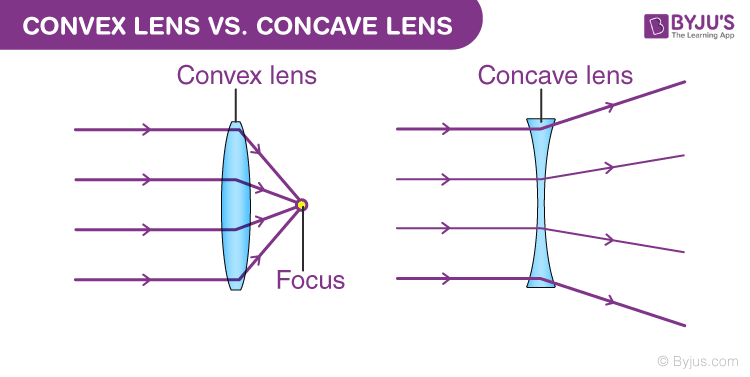
\includegraphics[width = \linewidth]{Convex-lens-1.png}
        \end{figure}
    \end{itemize}

    \section*{Relevant formula}
    \begin{enumerate}
        \item $P = \frac{1}{f}, \: power \, = \, \frac{1}{focal \, length}$
        \item $P = P_{1} + P_{2} + P_{3} + \ldots, \: total \, power \, = \, power \, of \, 
        lens \, 1 \,+\, power \, of \, lens \, 2 \, +\, \ldots$
        \item $\frac{1}{f} = \frac{1}{u} + \frac{1}{v}, \: \frac{1}{focal \, length} = 
        \frac{1}{object \, distance} + \frac{1}{image \, distance}$
        \item $m = \frac{v}{u}, \: magnification \, = \, \frac{image \, height}{object \, height}$
    \end{enumerate}

    \section*{Cases of ray diagrams}
    \subsection*{Case 1}
    Let's say we have a \textbf{converging} lens with object distance \textbf{further} than focal length.
    We get our normal diagram as lens has enough power to converge the \textbf{shallow} light rays hitting it.
    This is convex case 1 in the diagram below.

    \subsection*{Case 2}
    We have a \textbf{converging} lens with object distance \textbf{closer} than focal length.
    We get that our lens does not have enough power to converge the light rays as they are too
    \textbf{steep} and produces diverging light rays. This produces virtual image behind the object.
    This is convex case 2 in the diagram.

    \subsection*{Case 3}
    We have a \textbf{diverging} lens. This will produce a virtual image in between the object and the
    lens. This does not depend on whether the object is closer than the focal distance or further away
    from the lens.

    \begin{figure}[h]
        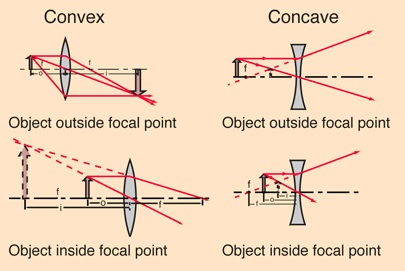
\includegraphics[scale = 1]{rayDiagCases.jpg} 
    \end{figure}

    
\end{document}